\section{Framework Components}
\label{sec:framework}
Current collaborative robot solutions guarantee safety, but they stop moving when an obstacle is detected rather than adapting the motion to display natural motions. The proposed dynamic obstacle avoidance solution is that of using obstacle detection to respond by moving around the obstacles while continuing to accomplish the desired tasks. Additionally, the integrated dynamic motion planning approach creates motion plans that fulfil various task specific constraints for typical industrial applications. For example the work cell 3D model is used to create a consistent model of the work environment, so that collision free trajectories are flexibly generated for different operations. The automatic consideration of these constraints drastically simplifies and speeds-up the deployment of the robot.

An artist's illustration of the proposed dynamic obstacle avoidance solution is shown in Fig. \ref{fig:overview}. The robot motion control component generates appropriate motion commands for the robot controller to follow the trajectories required for a given task. The proximity-sensing skin that covers the links and joints of the manipulator, produces information regarding potential collisions. This information is used by the robot motion control module to adapt the robot motions on the fly to fulfil both constraints: following the current trajectory (with a certain tolerance) and avoid collisions. If the collision is unavoidable with local deformations of the current trajectory, the robot motion control module requests a (global) re-planning,
which is performed on the fly by the reactive path-planner. The motion controller re-executes an alternate trajectory to achieve the final goal.
\begin{figure}[h]
\centering
{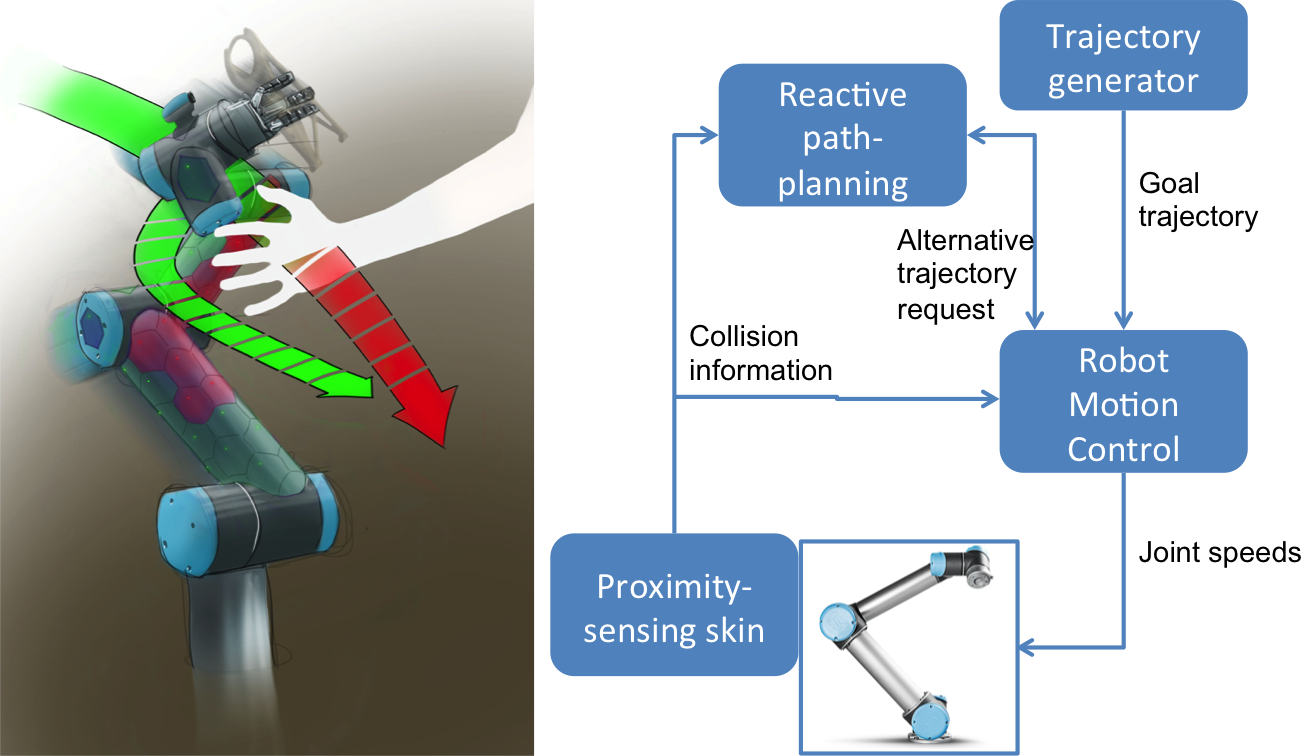
\includegraphics[scale=0.5]{chapters/doa/images/overview.png}}
\caption[0.1\textwidth]{An artist's schematization of the DOA
concept.}
\label{fig:overview}
\end{figure}
The figure \ref{fig:overview}(Left) shows the main idea of the framework which allows the robot arm to adapt its motion while executing a trajectory. The figure \ref{fig:overview}(Right) represents the pipeline of the framework used for collision avoidance and replanning. 
% \begin{figure}[h]
% \centering
% {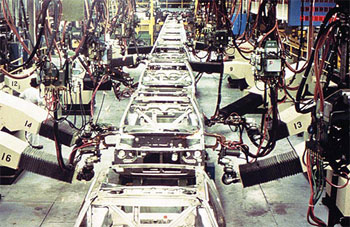
\includegraphics[scale=1]{intro/images/gm.jpg}}
% \caption{Manufacturing unit in General Motors with 'Unimate' robots in 1969}
% \label{fig:unimate}
% \end{figure}

\begin{figure}[h]
\centering
\resizebox{0.8\columnwidth}{!}{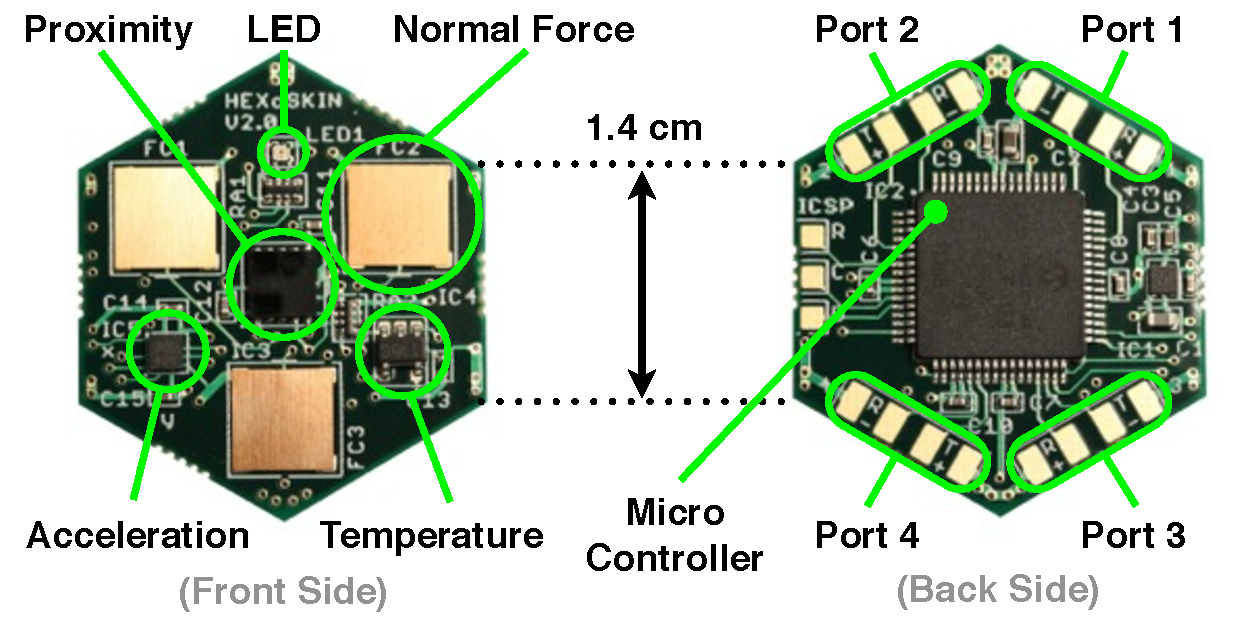
\includegraphics{chapters/doa/images/sensor_unit.pdf}}
\caption[]{Robot skin developed at Institute for Cognitive Systems, TUM.}
\label{fig:RobotSkin}
\vspace{-10pt}
\end{figure}	

\subsection{Artificial Robot Skin}
The development of \textit{Artificial Robot Skin}(ARS) is motivated by the necessity to provide robots with a rich and direct feedback of their interactions with the world. This system called as HEX-o-SKIN assembles multiple intelligent uniform unit cells with cell-2-cell communication allowing automatically cellular network organization \cite{mittendorfer2012uniform}. The robot skin system is modularized and transduces multi-modal tactile stimuli \cite{MittendorferYC15}. The robot skin consists of hexagonally shaped PCB modules called skin cells (see Fig. \ref{fig:RobotSkin}). A group of directly connected skin cells is termed skin patch. All skin cells are identical and contain the same set of sensors. The sensors sample 9 tactile stimuli of 4 different modalities, namely vibration (3D acceleration sensor), 3 normal forces (capacitive force sensor), 2 temperatures and 1 distance (optical proximity sensor). These sensors are either off-the-shelf standard ICs or in the case of the force sensors a in-house development. A micro-controller in the back of each skin cell collects data from its sensors, filters it and creates and sends data packets, which contain the most recent values of all sensors. All the skin cells are connected to each other via stretchable flex PCBs which allows the skin to cover curved surfaces and increases its robustness. The network of skin cells is a meshed bidirectional communication network which is routed by the micro-controllers of the skin cells. A self-organized algorithm initializes all the skin cells in a skin network and constructs a bidirectional communication path between each skin cell and the network root, the tactile section unit (TSU). The TSU converts skin network packets to standard UDP Ethernet packets and vice versa. This allows for fast low latency connections between robot skin and PC (see Fig. \ref{fig:SkinCellNetworkArchitecture}).
\begin{figure}[t]
\centering
\resizebox{0.8\columnwidth}{!}{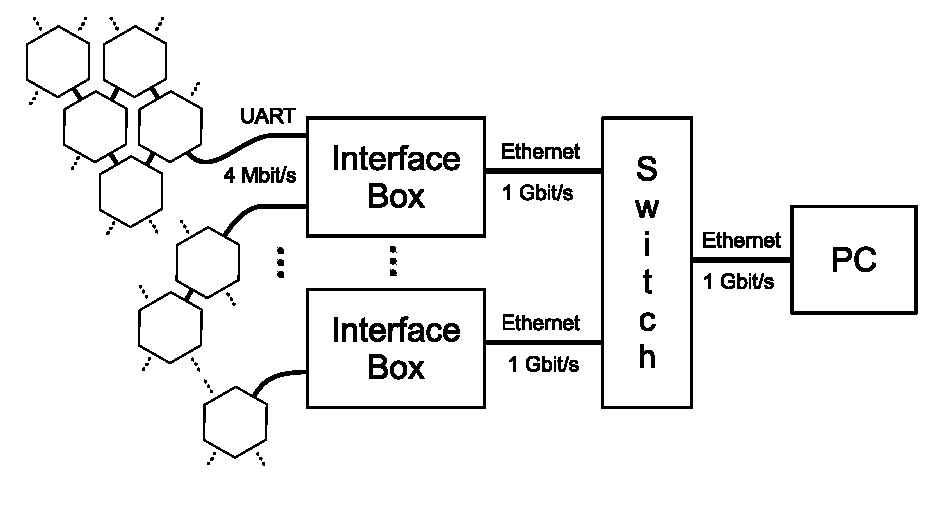
\includegraphics{chapters/doa/images/SkinCellNetwork.pdf}}\\[-15pt]
\caption[]{The skin cell network architecture and interface to the PC.}
\label{fig:SkinCellNetworkArchitecture}
\vspace{-10pt}
\end{figure}
The robot skin system also supports the auto-calibration of spatial relationships between skin cells of a skin patch covering a 3D surface \cite{Mittendorfer-IROS12tendorfer} such that the kinematic chain of every skin cell to the base frame can easily be determined. The proximity sensors used in the skin cells are infrared based sensors. The sensor emits infrared light and captures its reflections on obstacles in the range from 0 to 15 cm. The strength of the reflections allows the sensor to estimate the distance between the sensor and detected objects.  


\begin{figure}[h]
\centering
\resizebox{0.8\columnwidth}{!}{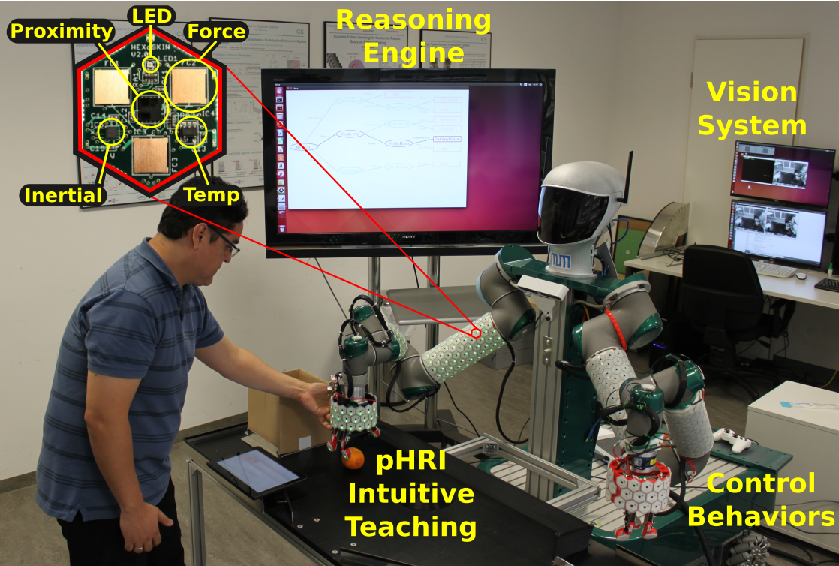
\includegraphics{chapters/doa/images/Demo.pdf}}\\[-10pt]
\caption[]{Robot TOMM with artificial robot skin.}
\label{fig:TommSorting}
\end{figure}

\paragraph{Evaluation of Artificial Robot Skin(ARS)}

The ARS has been successfully deployed on the robot TOMM \cite{Dean-ICRA17} (see Fig. \ref{fig:TommSorting}). The integration of the multi-modal artificial skin signals in the control loop of the arms is demonstrated in \cite{Dean-Humanoids16} where the self-calibrating artificial skin framework is used to control the dynamic behavior of the industrial robot, e.g. producing compliance in a non-compliant robot. The advantage of these compliant behaviors is to generate safer robots, especially for physical Human-Robot Interaction. The fusion of the multi-modal signals of the artificial skin with different sensors (e.g. cameras and joint encoders) in a semantic level is demonstrated in \cite{Ramirez-Amaro-Humanoids16}. These semantic representations are used to extract general task structures which together with the obtained knowledge can improve and accelerate teaching of new tasks \cite{Dynaov-Humanoids16}. Finally, the integration of these technologies has been evaluated in an industrial scenario, where a human can kinesthetically teach the robot TOMM to sort oranges \cite{Dean-IECON16} (see Fig. \ref{fig:TommSorting}). ARS has also been deployed successfully on another practical setup with a statically mounted Universal Robots UR5 robot (see Fig. \ref{fig:TUDSetup}). In this setup, the ARS is being used to provide proximity information related to obstacles in the immediate surroundings of the robot.

\begin{figure}[h]
\centering
\resizebox{0.8\textwidth}{!}{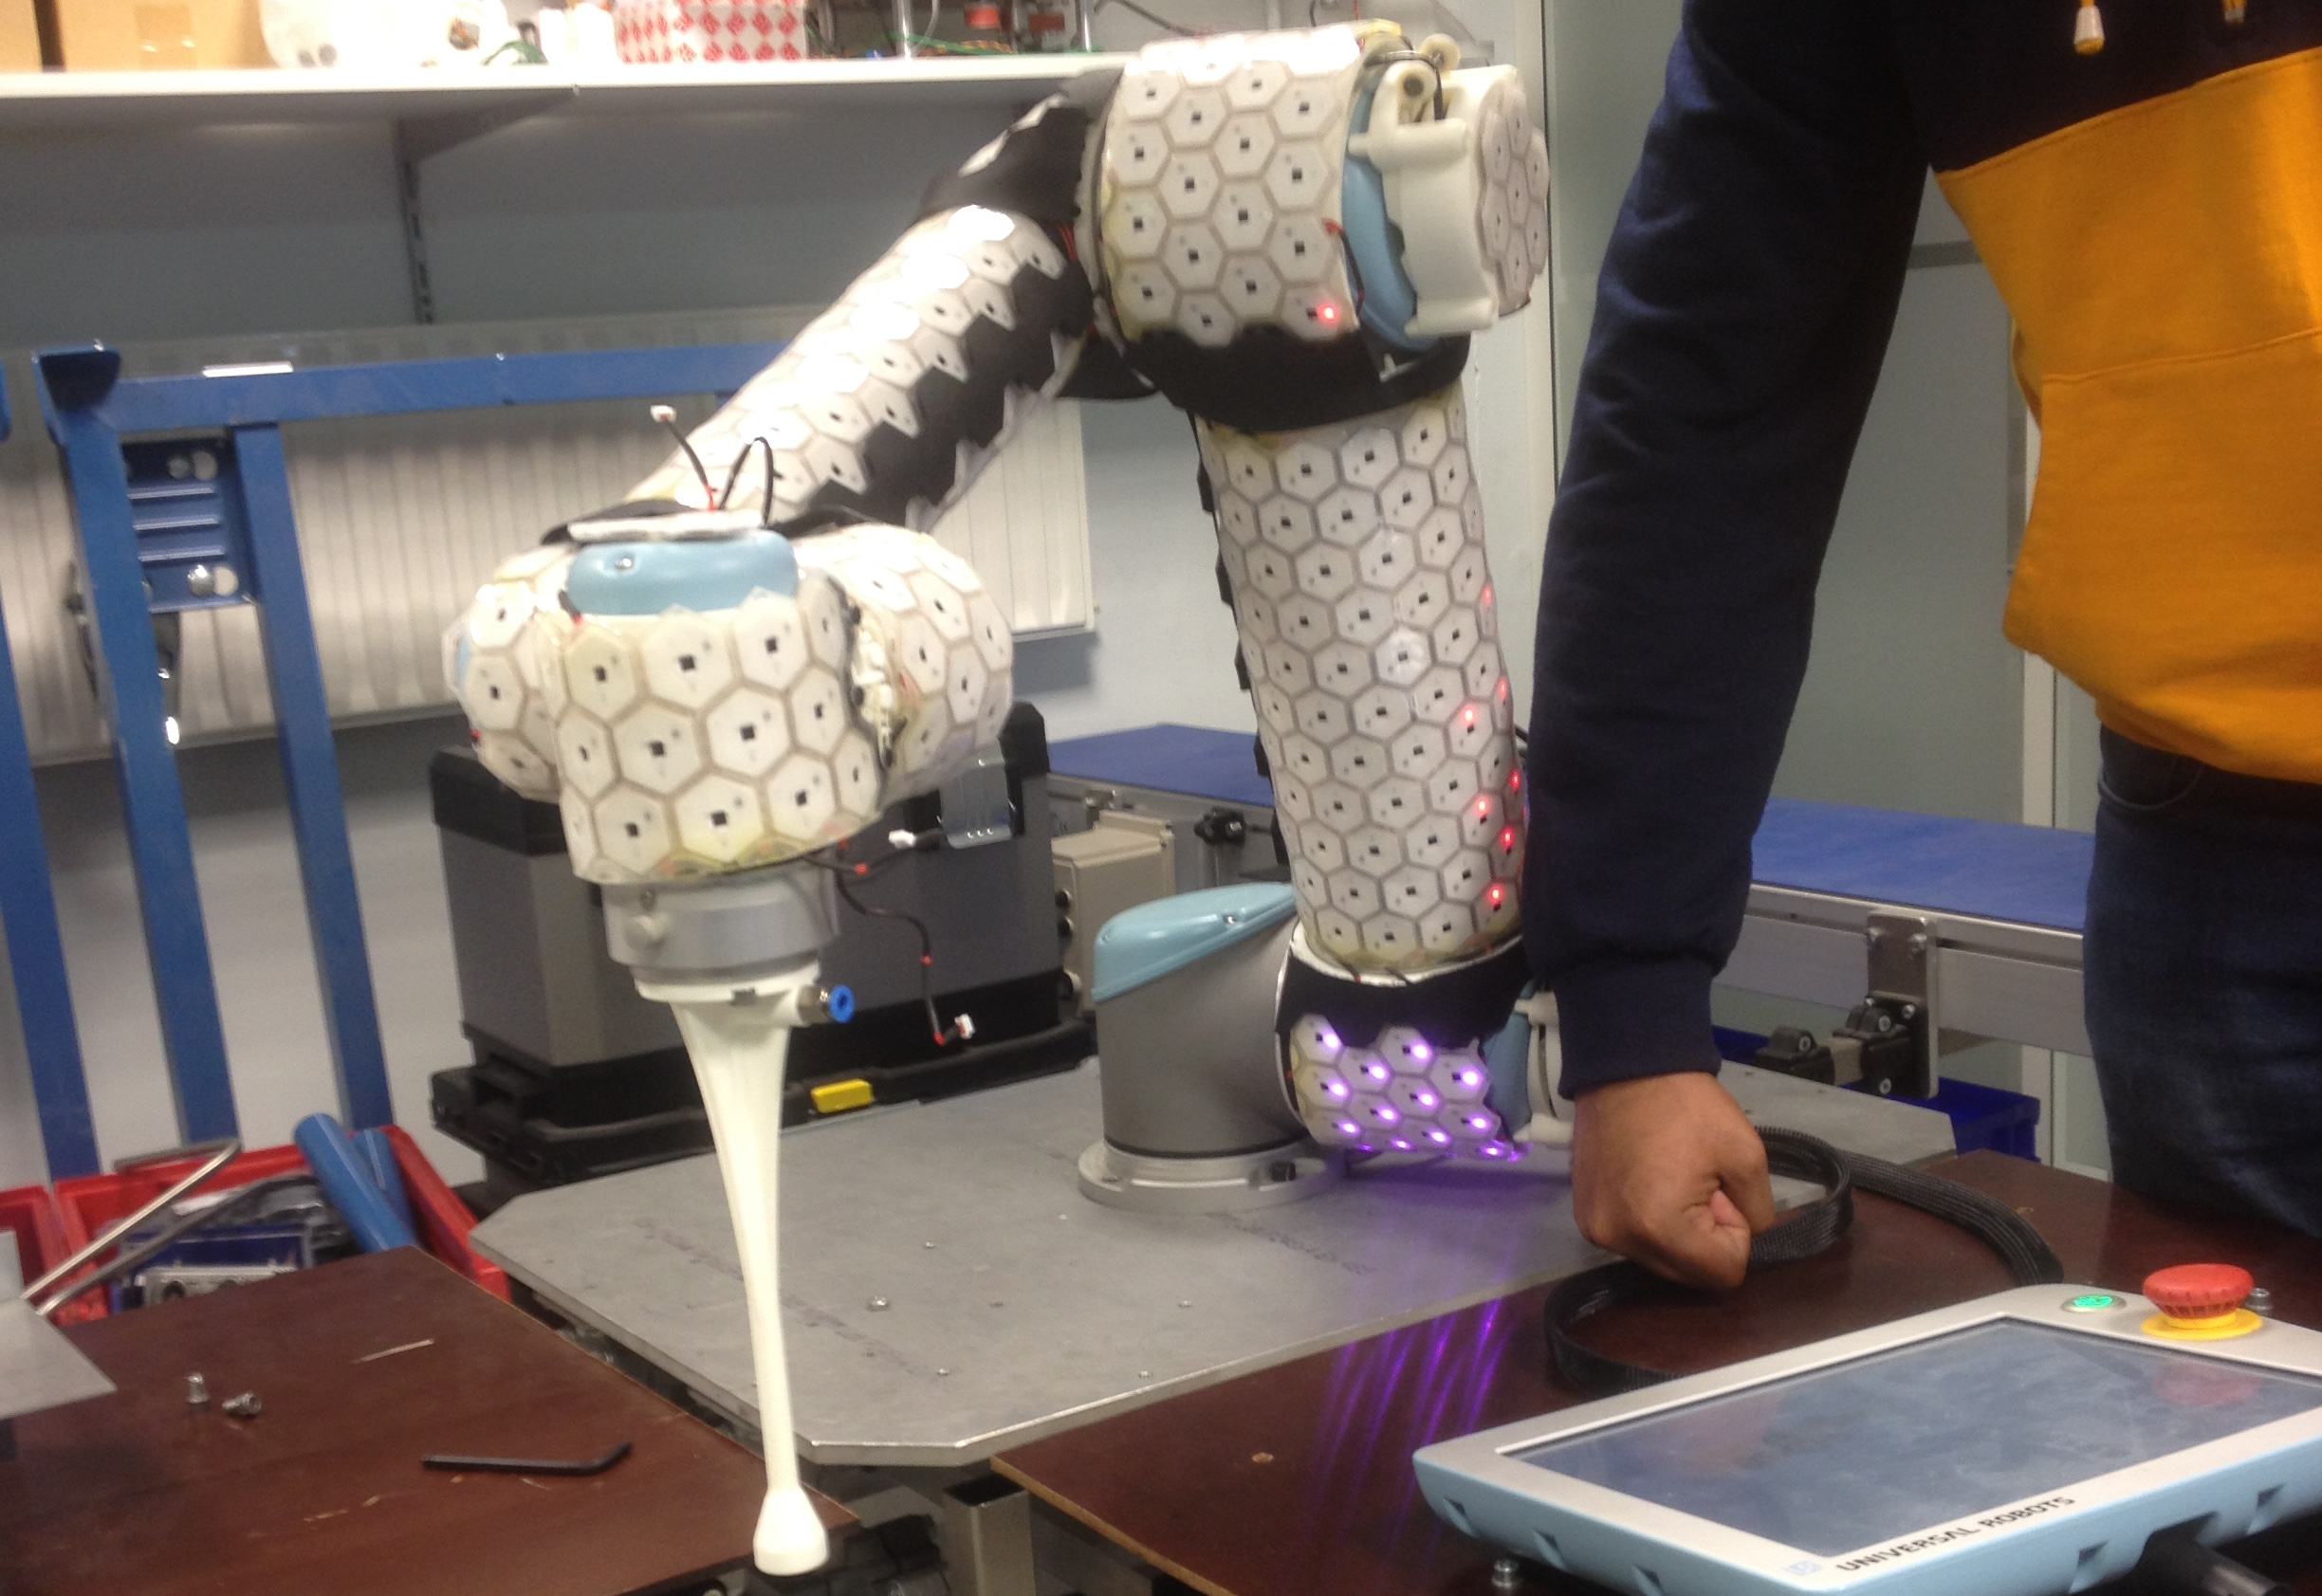
\includegraphics{chapters/doa/images/TUD_Setup.JPG}}\\[-10pt]
\caption[]{UR5 setup with Skin Cells activated (with red LEDs)}
\label{fig:TUDSetup}
\end{figure}


\subsection{Reactive Motion Planning}
\label{subsec:react_path}
\hypersetup{colorlinks, linkcolor=blue}
Though skin sensors can be used to reactively avoid obstacles locally, global aspect of the environment is necessary to avoid local minima, which is why we need an event based reactive replanner to help the controller in trouble. The reactive path planning component is developed by our partner Siemens, which is based on the industry grade KineoWorks\texttrademark\footnote{See
\href{http://www.plm.automation.siemens.com/en\_us/products/open/kineo/kineoworks/index.shtml}{Kineoworks}.} path planning library in order to provide fast and reliable robot paths. The intrinsic safety behaviors using torque/force sensing are reactive only after a collision has actually ocurred. This actually puts a constraint on the working velocity of the robot to be collaborative in industrial environments which we have pointed out earlier. The main motivation behind developing this component is to enable the robots to perform extrinsic safety behaviors which is quite inline with our goal to provide dynamic obstacle avoidance with appropriate caution. This component allows the robot to detect collisions in advance using depth information from Kinect camera and deform the trajectory by replanning in real time. The main advantage of using 3d sensors is to get a global view of the environment in contrast to proximity sensors on the surface of the robot which allows only local obstacle avoidance.

The complete collision avoidance component has been experimentally validated on a KUKA arm executing tasks in a environment with dynamic obstacles and a human operator. The reactive planner has been integrated with two trajectory generation frameworks: Reflexxes and Softmotion. Reflexxes \cite{kroger2011opening} framework can generate online time parameterized trajectories from a path. The generated jerk-limited and continuous trajectories takes into account of constraints on the dynamic robot capabilities with low latencies though there is no error bound between the reference and the executed trajectory.  The SoftMotion framework can generate online trajectories that limits jerk, acceleration and velocity for collaborative robot applications \cite{broquere2008soft,broquere2010motion}. The approach is based on the 7 segment acceleration profile by computing cubic curves for both point-point and continuous motions. The direct computation of the cubic parameters, the trajectory generator can be used on-line. Though it is incomplete as it cannot handle non-zero initial accelerations, it is experimentally validated and adapted for a KUKA LWR arm \cite{zhao2014online}. SoftMotion generates a trajectory with smoothing done at each stop point. The smoothed portion is constrained within a pre-defined tube respecting the error and kinematic bounds in real time making the trajectories more natural.



Actually, it is possible to use any trajectory generator as the planner generates a path as a polygonal line composed of a sequence of way points. For the proposed framework to avoid obstacles dynamically, we are only interested in the collision detection and the reactive planner module of this framework. The collision detection for dynamic obstacle avoidance is performed using the Kineo\texttrademark Collision Detector (KCD)\footnote{See \href{http://www.plm.automation.siemens.com/en\_us/products/open/kineo/collision-detector/index.shtml}{KCD}.}. KCD performs 3D collision detection and minimal distance analysis between triangular mesh surfaces in assembly environments. KCD has been designed specifically to minimize memory usage and take advantage of parallel processing. The component is synchronized with the OctoMap module which is updated at 30Hz with the point clouds acquired by an Xtion or Kinect camera sensors. Due to the necessity to perform reactive planning, the Octomap needs to be updated at higher rate which requires robust noise removal mechanisms. These filters removes Nan depth values and spurious points corresponding to noise, no-collision regions\& specular surfaces. The sparse outliers are removed using a statistical gaussian filter available in the PCL library \cite{rusu20113d}. The point cloud corresponding to robot links, joints and other bodies connected with the robot can be removed as well making the detection complete and flexible to be used in real time scenarios though the quality depends on a good hand-eye calibration.

\paragraph{Reactive path planning state machine}
Reactive path planning is done in the robot application node which coordinates the interaction between the path planning and the controller components executing the global tasks in real time. The path (re) planning strategy is implemented in the state machine as shown in the figure \ref{fig:KineoStates}.
\begin{itemize}
  \item \textbf{WAITING}: An idle state waiting for planning request.
  \item \textbf{PLANNING}: The controller requests the path planner node and waits for a collision free path composed of a sequence of way points. The controller executes a collision free trajectory by tracking the way points using Reflexxes or Soft Motion trajectory generator. In the proposed dynamic collision avoidance framework in the thesis, we use 'Stack of Tasks' to generate motions for a variety of reasons discussed in the next section.  In case the path planner fails due to nature of random tree algorithms, a fall back strategy to retry planning is implemented until a predefined timeout. The robot motion is cancelled in case no solutions exist.
  \item \textbf{MONITORING}: The trajectory execution by the robot is monitored for un-avoidable collisions. If the controller is intelligent enough to handle local collisions, the application node just monitors until the goal is reached. In case the obstacles doesn't allow for local path deformation, then the next state is triggered to replan.  
  \item \textbf{MONITORING WITH PLANNING PENDING}: An unavoidable collision is detected which has triggered to reach this state where the application node basically sends a new path planning request to the planner. Collisions are detected more accurately in this state as the reactive path planning considers the depth information represented in Octomap. The fast distance computation between the robot and environment using an efficient algorithm which is protected by Siemens, is used to reactively plan without creating any obstacle models which costs a lot of time.        
\end{itemize}

\begin{figure}[h]
\centering
\resizebox{1\textwidth}{!}{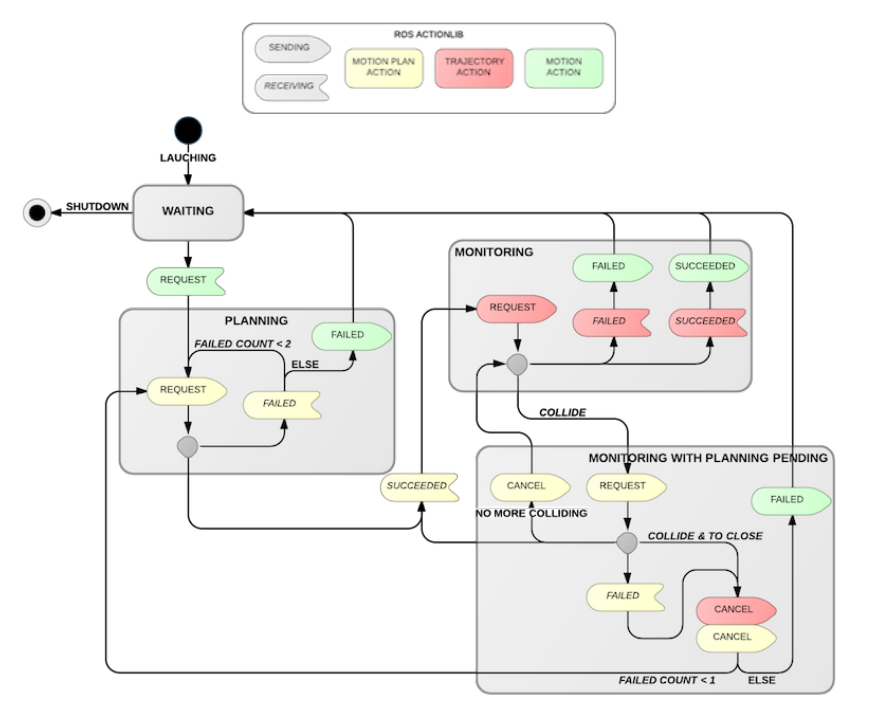
\includegraphics{chapters/doa/images/kineo_0.png}}\\[-10pt]
\caption[]{Reactive Path Planning State Machine}
\label{fig:KineoStates}
\end{figure}

This framework has been seamlessly integrated into the ROS-ecosystem via a ROS package called \texttt{kws\_ros\_interface} which provides the planner implementations of KineoWorks as shared objects that are readily usable in ROS-based software via the \texttt{kws\_ros\_planner} ROS node.Robot kinematic models are provided to KineoWorks in the Unified Robot Description Format (URDF) which is a ROS standard. Furthermore, KineoWorks also accepts the standard ROS representation of a \texttt{PointCloud}\footnote{See http://wiki.ros.org/pcl} for creating collision models of dynamic obstacles in the environment. 

\subsection{Reactive Controller}
The complete software architecture used for the Dynamic Collision Avoidance capability is shown in Fig. \ref{fig:arch_dca}. The motion control is achieved using the Stack of Tasks (SoT) controller framework \cite{Mansard2009} which employs a task based hierarchical jacobian control strategy eliminating the analytical inverse kinematics computation thus making it a generic controller for all robot platforms. 
The task function formalism is very well discussed in \cite{C.Samson1991}. A \emph{task} basically is a control law that achieves a specific objective which can be a free space task or just an inequality constraint that narrows down the workspace of the robot. The controller's hierarchical nature allows the robot to handle multiple kinematic tasks simultaneously exploiting the kinematic redundancy of the robot. The controller's real time capability comes from the high computational speed of the state of the art Hierarchical Quadratic Programming (HQP) solver backing it. In the context of our work, tasks generally include robot joint posture task, collision avoidance task, joint limits task and so on. The SoT framework handles the task priorities hierarchically in the real time to ensure there are no conflicts among tasks which is used to achieve dynamic obstacle avoidance without compromising on the main goal.

For example, let us consider a pick and place application in a collaborative environment. The primary goal for this application is to enable a robot to move to a (set of) desired pick and place locations repetitively. The pick and place locations can be defined as posture tasks in SoT. However, a higher priority task considering the collaborative nature of the environment is to avoid
collisions with obstacles that could be humans, for instance. Typically such a task is modelled as an ``Inequality'' task and an eventual feasible solution (if one exists) is computed by the solver by exploiting the kinematic redundancy of the robot. In the jargon of motion planning and control, this behavior is similar to a \emph{local planner}. However, it is likely that a feasible solution is not found due to the solver converging to a local minima\footnote{This is caused by the use of task Jacobians. For further details, please see \cite{Mansard2009}.} In such a scenario, SoT can also be used to leverage the services of a global planner (see Section \ref{subsec:react_path}) from the current robot state to the goal so that an entirely new path is obtained which is free from collisions and consequently allowing all the specified tasks to be achieved in the order of their priorities. The SoT controller has also been configured to work with the ROS-control interface. In all these setups, the proximity information from the artificial robot skin is used as an input to the collision avoidance task. In the following part, we briefly present the global path planner software framework that is used when the SoT controller hits a local minima.
\begin{figure}[t]
\centering
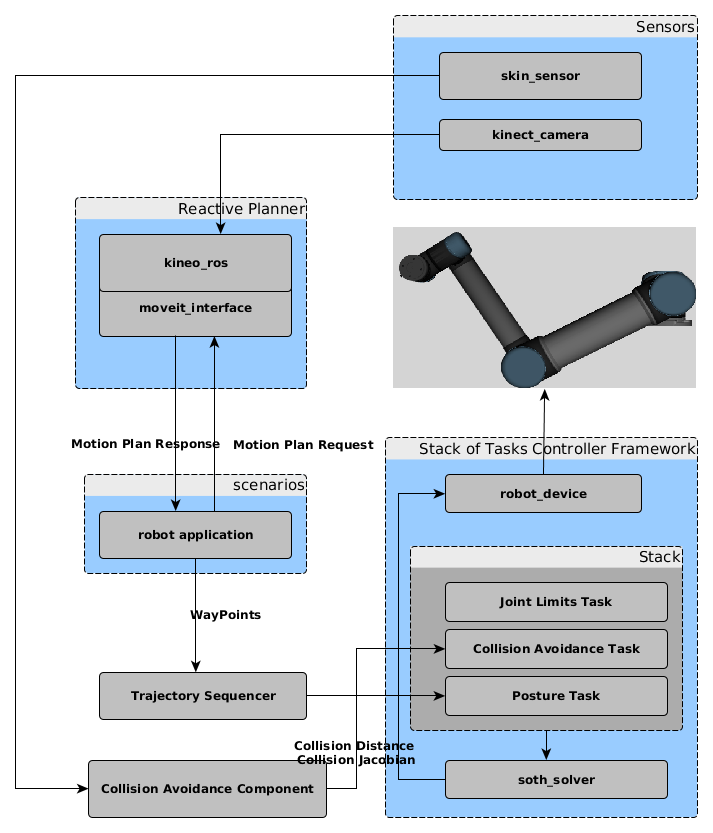
\includegraphics[scale=0.47]{chapters/doa/images/arch_dca.png}
\caption[]{Dynamic collision avoidance software architecture.}
\label{fig:arch_dca}
\end{figure}
